
\chapter*{Lecture 28}

\begin{recall}{}{}
\begin{itemize}
\item Next Monday: lecture swap with Prof Ghavam
\item Started with Laplace transforms
\end{itemize}
\end{recall}


\begin{figure}
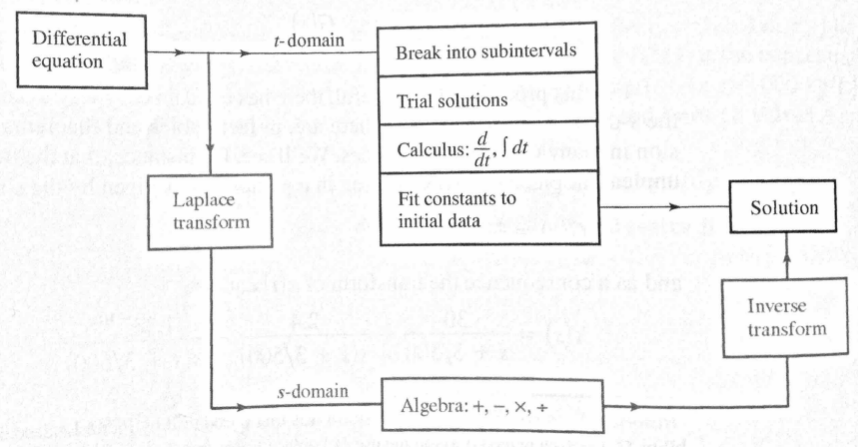
\includegraphics[width=\textwidth]{figs/LaplaceExample.png} 
\caption{Solution methods}
\end{figure}


RECALL:
\begin{equation}
\boxed{F(s)=\Lapl\left( f(t) \right) =\int^\infty_0 e^{-st} f(t) dt}
\end{equation}





Last lecture, we showed:
\begin{equation*}
=
\begin{cases}
   F(s)=\frac{1}{s^2} \qquad &\text{for } t\\
   F(s)=\frac{1}{s-\alpha}  &\text{for } e^{\alpha t} \text {when }>\alpha\\
   F(s)= ? &\text{for } e^{\cos \alpha t}
\end{cases}
\end{equation*}



\begin{exmp}{LT:}\\
Find the LT of $f(t)=\cos( \alpha t)$.\\
\textbf{Solution:}
\begin{align*}
\Lapl\left( f(t) \right) &=\int^\infty_0 e^{-st} \cos( \alpha t) dt\\
\end{align*}
We solve using integration by parts:
\begin{align*}
u &=e^{-st} \qquad \qquad & v=\frac{1}{\alpha} \sin(\alpha t)\\
du&=-s e^{-st}dt & dv=\cos(\alpha t) dt
\end{align*}
\begin{align*}
\Lapl\left( f(t) \right) &=\left[uv-\int v du\right]^\infty_0
&=\left[\frac{1}{\alpha} e^{-st}\sin( \alpha t)\right]^\infty_0-\frac{1}{\alpha}\int^\infty_0 \sin(\alpha t)(-s) e^{-st}dt
\end{align*}
\begin{itemize}
\item If $s>0$
\begin{align*}
 &=0+\frac{s}{\alpha}\int^\infty_0 e^{-st}\sin(\alpha t) dt
\end{align*}
We can apply an integration by parts again:
\begin{align*}
 &=0+\frac{s}{\alpha}\int^\infty_0 e^{-st}\sin(\alpha t) dt\\
 &=\left[-\frac{s}{\alpha^2}e^{-st}\cos(\alpha t)\right]^\infty_0+\frac{S}{\alpha^2} \int^\infty_0 \cos(\alpha t)(-s)e^{-st}dt\\
 F(s)&= \frac{s}{\alpha^2}-\frac{s^2}{\alpha^2}\underbrace{\int^\infty_0 \cos(\alpha t)e^{-st}dt}_{F(s)}
\end{align*}
we rearrange:
\begin{align*}
 \left(1+\frac{s^2}{\alpha^2}\right)F(s)= \frac{s}{\alpha^2}
\end{align*}
Or:
\begin{align*}
\boxed{ \Lapl(\cos(\alpha t) =F(s) =\frac{s}{\alpha^2+s^2}}
\end{align*}
\end{itemize}
\end{exmp}


\begin{figure}
\centering
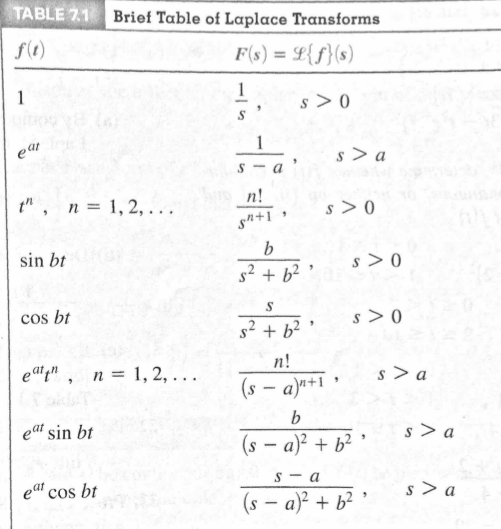
\includegraphics[width=0.7\textwidth]{figs/LaplaceIdentities.png}  
\caption{Laplace transforms}
\end{figure}


Question: how do we know that LT exists for a specific $f(t)$?
\section{Properties of the Laplace Transform}
\subsection{Existance of the LT}
For a given function $f(t)$, the Laplace transform will exist if the following two conditions :
\begin{itemize}
\item Piecewise continuous
\item Exponential order 
\end{itemize}
\subsubsection{Piecewise continuous:} A function $f(t)$ is piecewise continuous on $\left[0,\infty\right]$ if:
\begin{itemize}
\item the function is continuous except at a \textbf{finite} number of jump discontinuities.
\item $f(t)$ approaches a fi nite limit at each discontinuity.
\end{itemize}


\begin{figure}
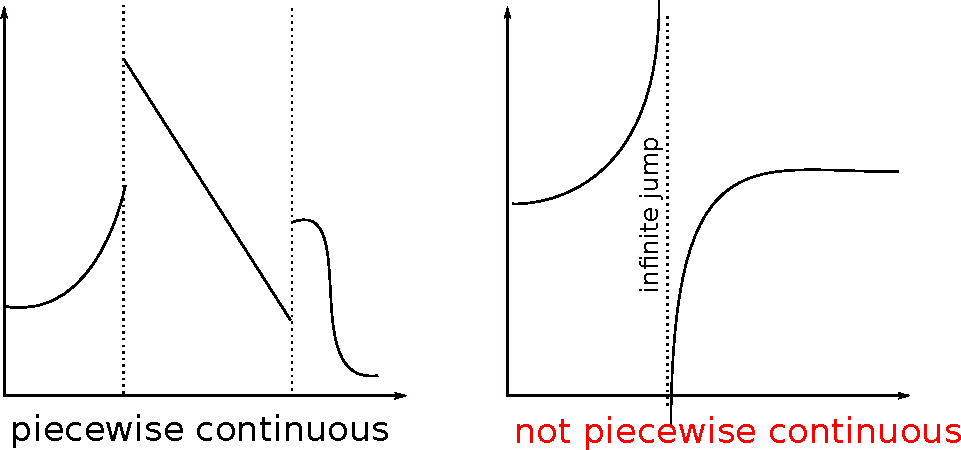
\includegraphics[width=\textwidth]{figs/piecewiseCont.pdf}
\caption{Piecewise continuity}
\end{figure}

\subsubsection{Exponential order:} In plain terms, the LT exists if the function does not grow faster than an exponential. A function $f(t)$ is said to be of exponential order $\alpha$ if there exist positive constants $T$ and $M$ such that:
\begin{equation*}
\left|f(t)\right|\leq Me^{\alpha t} \qquad \text{for all } t\geq T
\end{equation*}
\begin{exmp}{Exponential order:}\\
What is the exponential order of: $f(t)=e^{3t}\sin(2t)$\\
\textbf{Solution:} 
Since $\sin(2t)$ is bounded between -1 and 1:
\begin{equation*}
\left|e^{3t}\sin(2t)\right|\leq Me^{\alpha t} \qquad \text{for all } t\geq T
\end{equation*}
where $M=1$ and $T$ can take any value. The function is of exponential order $\alpha=3$.
\end{exmp}


\subsection{Linearity of  the transform}
Let $f$, $f_1$ and $f_2$be functions whose Laplace transforms exist for $s>\alpha$ and let $c$ be a constant. The linearity of the transform guarantees that:
\begin{align*}
&\Lapl (f_1+f_2)=\Lapl(f_1)+\Lapl(f_2)\\
&\Lapl (cf)=c\Lapl(f)
\end{align*}

Show the proof:
\begin{itemize}
\item 
\begin{align*}
\Lapl (f_1+f_2)&=\int^\infty_0 e^{-st}\left(f_1+f_2\right) dt\\
&=\int^\infty_0 e^{-st}f_1 dt+\int^\infty_0 e^{-st}f_2 dt\\
&=\Lapl(f_1)+\Lapl(f_2)
\end{align*}
\item 

\begin{align*}
\Lapl (cf)&=\int^\infty_0 e^{-st}\left(cf\right) dt\\
&=c\int^\infty_0 e^{-st}\left(f\right) dt\\
&=c\Lapl(f)
\end{align*}
\end{itemize}


\begin{exmp}{LT:}\\
Find the LT of :
\begin{equation*}
f(t)=
\begin{cases}
   2 \qquad &\text{for } 0<t<5\\
   0  &\text{for } 5<t<10 \\
   e^{4t} &\text{for } 10<t
\end{cases}
\end{equation*}
\textbf{Solution:}\\
\begin{enumerate}
\item Justify existance:
\begin{itemize}
\item Piecewise continuous? Yes (show drawing)
\item Of exponential order? Yes $\left|e^4t\right|\leq e^{4t}$ for $t>T=10$
\end{itemize}
\item Find LT:\\
\begin{align*}
F(s)=\Lapl(f(t))&=\int^\infty_0e^{-st}f(t) dt\\
&=\int^5_0e^{-st}2dt+\int^{10}_5 e^{-st} 0 dt + \int^\infty_{10} e^{-st} e^{4t}dt\\
&=-\frac{2}{s}\left[e^{-5s}-e^{0}\right]+0+\lim_{N\rightarrow \infty} \int^\infty_{10} e^{-(s-4)t}dt\\
&=\frac{2}{s}-\frac{2e^{-5s}}{5}+ \frac{e^{-10(s-4)}}{s-4} \qquad \text{for }s>4\\
\end{align*}

\end{enumerate}
\end{exmp}